\documentclass[12pt, a4paper]{article}

\usepackage[latin1]{inputenc}
\usepackage{tikz}
\usetikzlibrary{shapes,arrows}
\usetikzlibrary{positioning}
\usepackage{graphicx}
\usepackage{caption}
\usepackage{subcaption}
\begin{document}
\pagestyle{empty}


% % Define block styles
% \tikzstyle{decision} = [diamond, draw,
%     text width=4.5em, text badly centered, node distance=3cm, inner sep=0pt]
% \tikzstyle{block} = [rectangle, draw, 
%     text width=5em, text centered, rounded corners, minimum height=4em]
% \tikzstyle{line} = [draw, -latex']
% \tikzstyle{cloud} = [draw, ellipse, fill=red!20, node distance=3cm,
%     minimum height=2em]
    
% \begin{tikzpicture}[node distance = 2cm, auto]
%     % Place nodes
%     \node [block] (init) {initialize model};
%     \node [cloud, left of=init] (expert) {expert};
%     \node [cloud, right of=init] (system) {system};
%     \node [block, below of=init] (identify) {identify candidate models};
%     \node [block, below of=identify] (evaluate) {evaluate candidate models};
%     \node [block, left of=evaluate, node distance=3cm] (update) {update model};
%     \node [decision, below of=evaluate] (decide) {is best candidate better?};
%     \node [block, below of=decide, node distance=3cm] (stop) {stop};
%     % Draw edges
%     \path [line] (init) -- (identify);
%     \path [line] (identify) -- (evaluate);
%     \path [line] (evaluate) -- (decide);
%     \path [line] (decide) -| node [near start] {yes} (update);
%     \path [line] (update) |- (identify);
%     \path [line] (decide) -- node {no}(stop);
%     \path [line,dashed] (expert) -- (init);
%     \path [line,dashed] (system) -- (init);
%     \path [line,dashed] (system) |- (evaluate);
% \end{tikzpicture}

\begin{figure}[htp]
\centering
% \begin{subfigure}{.224 \textwidth}
%   \centering
%   \begin{tikzpicture}[scale=.75,every node/.style={minimum size=1cm},on grid]
%     \fill[gray, fill opacity=.8] (0.5,0) rectangle (2.5,2);
%     \begin{scope}[
%     	yshift=0,every node/.append style={
%     	    yslant=0.1,xslant=-0.1}
%     	             ]
%         \draw[step=5mm, black] (0,0) grid (4,2);
%         \draw[step=20mm, very thick, black] (0,0) grid (4,2);
%     \end{scope}
%     % \fill[red, fill opacity=.4] (0.5, 1.0) rectangle (1.0, 1.5);
%     % \draw[|<->|] (1.0, 1.25) to node {$d$} (2.0, 1.25);
%     \draw[line width=1.5pt] (2.0, 0.0) to (2.0, 2);
% \end{tikzpicture}
%   \caption{$\Delta t=1$}
%   \label{fig:t0}
% \end{subfigure}%
\begin{subfigure}{.224\textwidth}
  \centering
  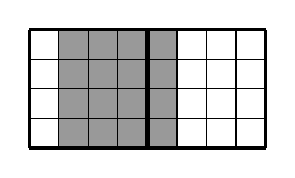
\begin{tikzpicture}[scale=.75,every node/.style={minimum size=1cm},on grid]
    \fill[gray, fill opacity=.8] (0.5,0) rectangle (2.5,2);
    \begin{scope}[
    	yshift=0,every node/.append style={
    	    yslant=0.1,xslant=-0.1}
    	             ]
        \draw[step=5mm, black] (0,0) grid (4,2);
        \draw[step=20mm, very thick, black] (0,0) grid (4,2);
    \end{scope}
    % \fill[red, fill opacity=.4] (0.5, 1.0) rectangle (1.0, 1.5);
    % \draw[|<->|] (1.0, 1.25) to node {$d$} (2.0, 1.25);
    \draw[line width=1.5pt] (2.0, 0.0) to (2.0, 2);
\end{tikzpicture}
  \caption{$\Delta t=1$}
  \label{fig:t0}
\end{subfigure}%
\hspace{1pt}
\begin{subfigure}{.224\textwidth}
  \centering
  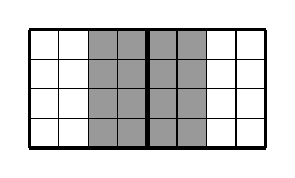
\begin{tikzpicture}[scale=.75,every node/.style={minimum size=1cm},on grid]
    \fill[gray, fill opacity=.8] (1.0,0) rectangle (3.0,2);
    \begin{scope}[
    	yshift=0,every node/.append style={
    	    yslant=0.1,xslant=-0.1}
    	             ]
        \draw[step=5mm, black] (0,0) grid (4,2);
        \draw[step=20mm, very thick, black] (0,0) grid (4,2);
    \end{scope}
    % \fill[green, fill opacity=.8] (3.0, 1.0) rectangle (3.5, 1.5);
    % \draw[|<->|] (2.0, 1.25) to node {$d$} (3.0, 1.25);
    \draw[line width=1.5pt] (2.0, 0.0) to (2.0, 2);
\end{tikzpicture}
  \caption{$\Delta t=2$}
  \label{fig:t1}
\end{subfigure}
\begin{subfigure}{.224\textwidth}
  \centering
  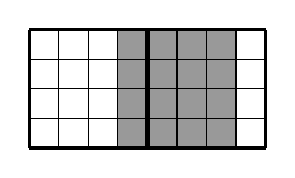
\begin{tikzpicture}[scale=.75,every node/.style={minimum size=1cm},on grid]
    \fill[gray, fill opacity=.8] (1.5,0) rectangle (3.5,2);
    \begin{scope}[
    	yshift=0,every node/.append style={
    	    yslant=0.1,xslant=-0.1}
    	             ]
        \draw[step=5mm, black] (0,0) grid (4,2);
        \draw[step=20mm, very thick, black] (0,0) grid (4,2);
    \end{scope}
    % \fill[red, fill opacity=.4] (0.5, 1.0) rectangle (1.0, 1.5);
    % \draw[|<->|] (1.0, 1.25) to node {$d$} (2.0, 1.25);
    \draw[line width=1.5pt] (2.0, 0.0) to (2.0, 2);
\end{tikzpicture}
  \caption{$\Delta t=3$}
  \label{fig:t2}
\end{subfigure}%
\hspace{1pt}
\begin{subfigure}{.224\textwidth}
  \centering
  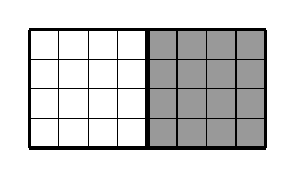
\begin{tikzpicture}[scale=.75,every node/.style={minimum size=1cm},on grid]
    \fill[gray, fill opacity=.8] (2.0,0) rectangle (4.0,2);
    \begin{scope}[
    	yshift=0,every node/.append style={
    	    yslant=0.1,xslant=-0.1}
    	             ]
        \draw[step=5mm, black] (0,0) grid (4,2);
        \draw[step=20mm, very thick, black] (0,0) grid (4,2);
    \end{scope}
    % \fill[green, fill opacity=.8] (3.0, 1.0) rectangle (3.5, 1.5);
    % \draw[|<->|] (2.0, 1.25) to node {$d$} (3.0, 1.25);
    \draw[line width=1.5pt] (2.0, 0.0) to (2.0, 2);
\end{tikzpicture}
  \caption{$\Delta t=4$}
  \label{fig:t3}
\end{subfigure}
\caption{
% The change of a flow from a node to one of its neighbors (right neighbor) along with the attacker's time step with $s=4$. The gray nodes are covered by the flow at each attacker's time step. Besides, the red (green) node is one of the node of the defender's grid where the flow flows out (in) and the corresponding distance $d=2$, defined in Algorithm~\ref{alg:mapping}, to the edge where the flow passes is displayed.
% TODO Find sources for these pictures.
}
\label{fig:mapping}
\end{figure}

\begin{figure}[htp]
\centering
% \begin{subfigure}{.224 \textwidth}
%   \centering
%   \begin{tikzpicture}[scale=.75,every node/.style={minimum size=1cm},on grid]
%     \fill[gray, fill opacity=.8] (0.5,0) rectangle (2.5,2);
%     \begin{scope}[
%     	yshift=0,every node/.append style={
%     	    yslant=0.1,xslant=-0.1}
%     	             ]
%         \draw[step=5mm, black] (0,0) grid (4,2);
%         \draw[step=20mm, very thick, black] (0,0) grid (4,2);
%     \end{scope}
%     % \fill[red, fill opacity=.4] (0.5, 1.0) rectangle (1.0, 1.5);
%     % \draw[|<->|] (1.0, 1.25) to node {$d$} (2.0, 1.25);
%     \draw[line width=1.5pt] (2.0, 0.0) to (2.0, 2);
% \end{tikzpicture}
%   \caption{$\Delta t=1$}
%   \label{fig:t0}
% \end{subfigure}%
\begin{subfigure}{.224\textwidth}
  \centering
  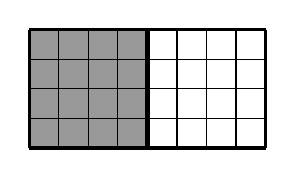
\begin{tikzpicture}[scale=.75,every node/.style={minimum size=1cm},on grid]
    \fill[gray, fill opacity=.8] (0,0) rectangle (2,2);
    \begin{scope}[
    	yshift=0,every node/.append style={
    	    yslant=0.1,xslant=-0.1}
    	             ]
        \draw[step=5mm, black] (0,0) grid (4,2);
        \draw[step=20mm, very thick, black] (0,0) grid (4,2);
    \end{scope}
    % \fill[red, fill opacity=.4] (0.5, 1.0) rectangle (1.0, 1.5);
    % \draw[|<->|] (1.0, 1.25) to node {$d$} (2.0, 1.25);
    \draw[line width=1.5pt] (2.0, 0.0) to (2.0, 2);
\end{tikzpicture}
  \caption{$T=1$}
  \label{fig:t01}
\end{subfigure}%
\hspace{1pt}
\begin{subfigure}{.224\textwidth}
  \centering
  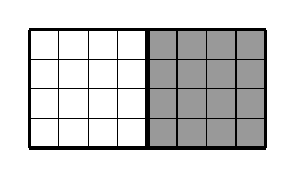
\begin{tikzpicture}[scale=.75,every node/.style={minimum size=1cm},on grid]
    \fill[gray, fill opacity=.8] (2.0,0) rectangle (4.0,2);
    \begin{scope}[
    	yshift=0,every node/.append style={
    	    yslant=0.1,xslant=-0.1}
    	             ]
        \draw[step=5mm, black] (0,0) grid (4,2);
        \draw[step=20mm, very thick, black] (0,0) grid (4,2);
    \end{scope}
    % \fill[green, fill opacity=.8] (3.0, 1.0) rectangle (3.5, 1.5);
    % \draw[|<->|] (2.0, 1.25) to node {$d$} (3.0, 1.25);
    \draw[line width=1.5pt] (2.0, 0.0) to (2.0, 2);
\end{tikzpicture}
  \caption{$T=2$}
  \label{fig:t11}
\end{subfigure}
\caption{
% The change of a flow from a node to one of its neighbors (right neighbor) along with the attacker's time step with $s=4$. The gray nodes are covered by the flow at each attacker's time step. Besides, the red (green) node is one of the node of the defender's grid where the flow flows out (in) and the corresponding distance $d=2$, defined in Algorithm~\ref{alg:mapping}, to the edge where the flow passes is displayed.
% TODO Find sources for these pictures.
}
\label{fig:mapping1}
\end{figure}

\end{document}